\section{Sequences}
  A \textbf{sequence} can be thought of as a list of numbers written in a definite order:
  $$a_1,\ a_2,\ a_3,\ a_4,\ \ldots,\ a_n,\ \ldots$$
  The number $a_1$ is the \textit{first term}, $a_2$ is the \textit{second term}, and in general $a_n$ is the \textit{nth term}. We will deal with infinite sequences exclusively so each term $a_n$ will have a successor $a_n+1$.\par
  Notice that for every positive integer $n$ there is a corresponding number $a_n$ so a sequence can be defined as a function whose domain is the set of positive integers. We usually write $a_n$ instead of the function notation $f(n)$.
  \begin{center}
  \uppercase{Notation}\quad The sequence ${a_1,\ a_2,\ a_3,\ \ldots}$ is also denoted by
  $${a_n}\quad \text{or}\quad {a_n}_{n=1}^{\infty}$$
  \end{center}
  \begin{example}
    Some sequences can be defined by giving a formula for the \textit{n}th term. In this example, we will describe a sequence in 3 ways: the previous notation, defining a formula, and writing out the terms of the sequence. Note that $n$ doesn't have to start at 1.
    \begin{enumerate}
      \item $$\left\{\frac{n}{n+1}\right\}_{n=1}^{\infty} \quad a_n=\frac{n}{n+1}\quad \left\{\frac{1}{2},\ \frac{2}{3},\ \frac{3}{4},\ \frac{4}{5},\ldots,\ \frac{n}{n+1},\ldots\right\}$$
      \item $$\left\{\frac{(-1)^n (n+1)}{3^n}\right\} \quad a_n=\frac{(-1)^n (n+1)}{3^n}\quad \left\{-\frac{2}{3},\ \frac{3}{9},\ -\frac{4}{27},\ \frac{5}{81},\ldots,\ \frac{(-1)^n (n+1)}{3^n},\ldots\right\}$$
      \item $$\{\sqrt{n-3}\}_{n=3}^{\infty} \quad a_n=\sqrt{n-3},\ n\geq3 \quad \{0,\ 1,\ \sqrt{2},\ \sqrt{3},\ldots,\ \sqrt{n-3},\ldots\}$$
      \item $$\left\{\cos{\frac{n\pi}{6}}\right\}_{n=0}^{\infty} \quad a_n=\cos{\frac{n\pi}{6}},\ n\geq0 \quad \left\{1,\ \frac{\sqrt{3}}{2},\ \frac{1}{2},\ 0,\ldots,\ \cos{\frac{n\pi}{6}},\ldots\right\}$$
    \end{enumerate}
  \end{example}
  \begin{example}
    Find a formula for the general term $a_n$ of the sequence $$\left\{\frac{3}{5},\ -\frac{4}{25},\ \frac{5}{125},\ -\frac{6}{625},\ \frac{7}{3125},\ldots\right\}$$
  \end{example}
  \begin{solution}
    We are given the first five terms. The numerator of the fractions start at 3 and increase by 1, so the nth term will have numerator $n+1$. The demoninators are the powers of 5, so $a_n$ has denominator $5^n$. The signs of the terms alternate between positive and negative, so we need to multiply by a power of 1. The factor $(-1)^n$ means we start with a negative term, so here we use $(-1)^{n-1}$ or $(-1)^{n+1}$ because we start with a positive term. Therefore,
    $$a_n=(-1)^{n-1}\frac{n+2}{5^n}$$
  \end{solution}
  \begin{definition}
    A sequence $\{a_n\}$ has the \textbf{limit} $L$ and we write
    $$\lim_{n\to\infty} a_n = L \qquad \text{or} \qquad a_n \to L\ \text{as}\ n \to \infty$$
    if we can make the terms $a_n$ as close to $L$ as wel like by taking $n$ sufficiently large. If $lim_{n \to \infty} a_n$ exists, we say the sequence \textbf{converges} (or is \textbf{convergent}). Otherwise, we say the sequence \textbf{diverges} (or is \textbf{divergent}).
  \end{definition}
  The figure below graphs examples of two sequences that have the limit $L$.
  \begin{center}
    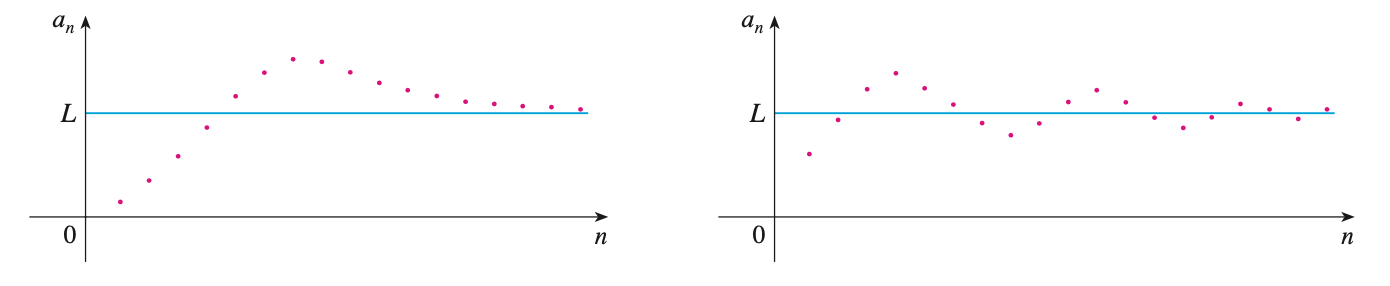
\includegraphics[width=\textwidth]{limit_of_sequence_example.png}
  \end{center}
  A more precise version of the previous definition is
  \begin{definition}
    A sequence $\{a_n\}$ has the \textbf{limit} $L$ and we write
    $$\lim_{n\to\infty} a_n = L \qquad \text{or} \qquad a_n \to L\ \text{as}\ n \to \infty$$
    if for every $\varepsilon > 0$ there is a corresponding integer $N$ such that
    $$|a_n - L| < \varepsilon \quad \text{whenever } n > N$$
  \end{definition}
  No matter how small an interval $(L-\varepsilon\ L+\varepsilon)$ is chosen, there exists an $N$ such that all terms of the sequence from $a_{N+1}$ onward must lie in that interval.
  \begin{center}
    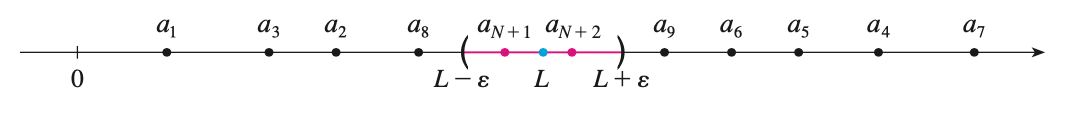
\includegraphics[width=\textwidth]{number_line.png}
  \end{center}
  The points on the graph of $a_n$ must lie between the horizontal lines $y=L+\varepsilon$ and $y=L-\varepsilon$ if $n > N$. This picture must be valid no matter how small $\varepsilon$ is chosen, but usually a smaller $\varepsilon$ requires a larger $N$.
  \begin{center}
    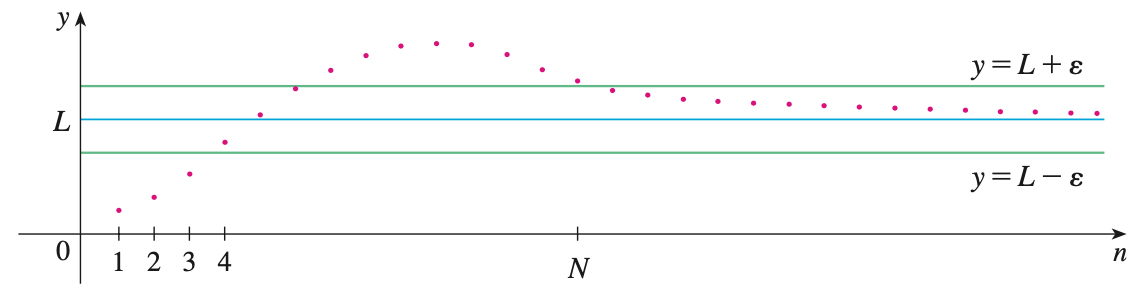
\includegraphics[width=\textwidth]{sequence_convergence.png}
  \end{center}
  The only difference between $\lim\limits_{n \to \infty} a_n = L$ and $\lim\limits_{x \to \infty} f(x) = L$ is that $n$ is required to be an integer.
  \begin{theorem}
    If $\lim\limits_{x \to \infty} f(x) = L$ and $f(n)=a_n$ when $n$ is an interger, then $\lim_{n \to \infty} = a_n = L$.
  \end{theorem}
  Since we know that $\lim\limits_{x \to \infty} (1/x^r)=0$ when $r>0$, we can use the previous theorem to get
  \begin{definition}
    $$\lim_{n \to \infty} \frac{1}{n^r}=0 \quad \text{if}\ r>0$$
  \end{definition}
  If $a_n$ grows as $n$ grows, we use the notation $\lim_{n \to \infty} a_n = \infty$. We say that $a_n$ diverges to $\infty$.
  \begin{definition}
    $\lim_{n \to \infty} a_n = \infty$ means that for every positive number $M$ there is an integer $N$ such that
    $$a_n>M \quad \text{whenever}\ n>N$$
  \end{definition}
  \begin{definition}[\textbf{Limit Laws for Sequences} (similar to original Limit Laws)]
    If $\{a_n\}$ and $\{b_n\}$ are convergent sequences and $c$ is a constant, then
   \begin{itemize}
     \item[] $\lim\limits_{n \to \infty} (a_n + b_n) = \lim\limits_{n \to \infty} a_n + \lim\limits_{n \to \infty} b_n$
     \item[] $\lim\limits_{n \to \infty} (a_n - b_n) = \lim\limits_{n \to \infty} a_n - \lim\limits_{n \to \infty} b_n$
     \item[] $\lim\limits_{n \to \infty} ca_n = c\lim\limits_{n \to \infty} a_n$ \hspace{100pt} $\lim\limits_{n \to \infty} c = c$
     \item[] $\lim\limits_{n \to \infty} (a_n b_n) = \lim\limits_{n \to \infty} a_n \cdot \lim\limits_{n \to \infty} b_n$
     \item[] $\lim\limits_{n \to \infty} \frac{a_n}{b_n} = \frac{\lim\limits_{n \to \infty} a_n}{\lim\limits_{n \to \infty} b_n} \quad \text{if}\ b_n \neq 0$
     \item[] $\lim\limits_{n \to \infty} (a_{n}^{p}) = \left[\lim\limits_{n \to \infty} a_n\right]^p \quad \text{if}\ p > 0\ \text{and}\ a_n > 0$
   \end{itemize}
  \end{definition}
  \begin{theorem}[\textbf{The Squeeze Theorem for Sequences} (same as original)]
    If $a_n \leq b_n \leq c_n$ for $n \geq n_0$ and $\lim\limits_{n \to \infty} a_n = \lim\limits_{n \to \infty} c_n = L$, then $\lim\limits_{n \to \infty} b_n = L$.
  \end{theorem}
  \begin{center}
    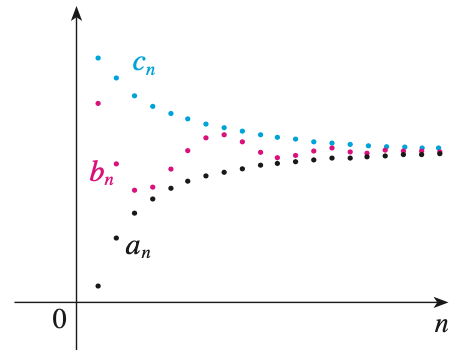
\includegraphics[width=200px]{squeeze.png}
  \end{center}
  \begin{theorem}
    If $\lim\limits_{n\to\infty}|a_n| = 0, then \lim\limits_{n\to\infty}a_n = 0$.
  \end{theorem}
  \begin{example}
    Evaluate $\lim\limits_{n\to\infty}\frac{(-1)^n}{n}$ if it exists.
  \end{example}
  \begin{solution}
    $$\lim_{n\to\infty}\left|\frac{(-1)^n}{n}\right|=\lim_{n\to\infty}\frac{1}{n}=0 \quad \text{so}\ \lim_{n\to\infty}\frac{(-1)^n}{n}=0$$
  \end{solution}
  \begin{example}
    Find $\lim\limits_{n \to \infty} \frac{n}{n+1}$.
  \end{example}
  \begin{solution}
    Divide the numberator and denominator by the highest power of $n$ and then use the Limit Laws.
    \begin{align*}
        \lim_{n \to \infty} \frac{n}{n+1} &= \lim_{n \to \infty} \frac{1}{1+\frac{1}{n}} = \frac{\lim\limits_{n \to \infty} 1}{\lim\limits_{n \to \infty}1+\lim\limits_{n \to \infty}\frac{1}{n}} \\
        &= \frac{1}{1+0}=1
    \end{align*}
  \end{solution}
  \begin{example}
    Calculate $\lim\limits_{n \to \infty} \frac{\ln n}{n}$.
  \end{example}
  \begin{solution}
    Both the numerator and demoninator approach infinity as $n\to\infty$. We can't apply l'Hospital;s Rule directly because it applies to functions, not sequences. However, we can apply it to the related function.
    \begin{equation*}
        \lim_{x \to \infty} \frac{\ln x}{x} = \lim_{x \to \infty} \frac{1/x}{1} = 0 \quad \text{so}\ \lim\limits_{n \to \infty} \frac{\ln n}{n} = 0
    \end{equation*}
  \end{solution}
  \begin{example}
    Determine whether the sequence $a_n = (-1)^n$ is convergent or divergent.
  \end{example}
  \begin{solution}
    If we write out the terms of the sequence, we get $\{-1,\ 1,\ -1,\ 1,\ -1,\ 1,\ -1,\ldots\}$. Since the terms oscillate between 1 and -1, $a_n$ does not approach any number. Thus, $\lim_{n\to\infty}(-1)^n$ does not exist so the sequence $\{(-1)^n\}$ is divergent.
  \end{solution}
  \begin{example}
    Discuss the convergence of the the sequence $a_n=n!/n^n$.
  \end{example}
  \begin{solution}
    Both the numerator and denominator approach infinity as $n\to\infty$, but we have no corresponding functions to use l'Hospital's Rule because $x!$ is not defined when $x$ is not an integer. if we write the general forumula for the sequence, we get
    $$a_n = \frac{1\cdot2\cdot3\cdot\ldots\cdot n}{n\cdot n\cdot n\cdot\ldots\cdot n} = \frac{1}{n}\left(\frac{2\cdot3\cdot\ldots\cdot n}{n\cdot n\cdot n\cdot\ldots\cdot n}\right)$$
    The expression in the parenthesis is at most 1 because the numerator is less than (or equal) to the denominator, so
    $$0<a_n \leq \frac{1}{n}$$
    We can use the squeeze theorem because both 0 and $1/n$ $\to$ 0 as $n\to\infty$, so $a_n \to \infty$ as $n\to\infty$.
  \end{solution}
  \begin{example}
    Determine if the sequences below converge. If they do, find the limits as $n\to\infty$.
    \begin{enumerate}
      \item $\frac{\sin n}{n}$
      \item $ne^{-n}$
    \end{enumerate}
  \end{example}
  \begin{solution}
    \begin{enumerate}
      \item $\frac{\sin n}{n}$ converges to 0 by the squeeze theorem
            \begin{gather*}
               -\frac{1}{n}\leq\frac{\sin n}{n}\leq-\frac{1}{n}\ \text{,}\ \lim_{n\to\infty}\frac{1}{n}=0\ \text{, so} \\
               0 \leq\frac{\sin n}{n}\leq 0 \implies \lim_{n\to\infty}\frac{\sin n}{n}=0
            \end{gather*}
      \item $ne^{-n} = \frac{n}{e^n}$. The denominator $e^n$ converges faster than the numerator $n$ does. Use l'Hospital's Rule to get $$\lim_{x\to\infty}\frac{x}{e^x} = \lim_{x\to\infty}\frac{1}{e^x} = 0\ \text{so}\ \lim_{n\to\infty}ne^{-n} = 0$$
    \end{enumerate}
  \end{solution}
  \begin{example}
    Show that if $\lim\limits_{n \to \infty}a_{2n} = L$ and $\lim\limits_{n \to \infty}a_{2n+1} = L$, $\{a_n\}$ is convergent and $\lim\limits_{n \to \infty}a_n = L$.
  \end{example}
  \begin{solution}
    The solution uses the symbols $\exists$ ("exists") and $\implies$ ("implies").
    \begin{align*}
      \text{Since}\ &\lim\limits_{n \to \infty}a_{2n} = L\text{, }\quad&& \exists\ N_1 \implies |a_{2n}-L|<\varepsilon\ \text{for}\ n>N_1 \\
      \text{Since}\ &\lim\limits_{n \to \infty}a_{2n+1} = L\text{, }\quad&& \exists\ N_2 \implies |a_{2n+1}-L|<\varepsilon\ \text{for}\ n>N_2
    \end{align*}
    Let $N=\max\{2N_1,2N_2 + 1\}$ and let $n>N$.
    \begin{align*}
      &\text{If $n$ is even, }\quad &&n=2m \text{, } m>N_1 \text{, } |a_n - L| = |a_{2m}-L|<\varepsilon \\
      &\text{If $n$ is odd, }\quad &&n=2m+1 \text{, } m>N_2 \text{, } |a_n - L| = |a_{2m+1}-L|<\varepsilon \\
    \end{align*}
    Therefore, $\{a_n\}$ is convergent and $\lim\limits_{n \to \infty}a_n=L$.
  \end{solution}
  \begin{definition}
    The sequence $\{r^n\}$ is convergent if $-1<r\leq1$ and divergent for all other values of $r$.
    $$ \lim_{n \to \infty} r^n =
    \begin{cases}
      0 &\text{if } -1<r<1 \\
      0 &\text{if } r=1
    \end{cases}$$
  \end{definition}
  \begin{definition}
    A sequence $\{a_n\}$ is \textbf{increasing} if $a_n < a_{n+1}$ for all $n\geq 1$ $(a_1 < a_2 < a_3 < \cdots)$. It is \textbf{decreasing} is $a_n < a_{n+1}$ for all $n\geq 1$. It is \textbf{monotonic} if the is either increasing or decreasing.
  \end{definition}
  \begin{example}
    The sequence $\left\{\frac{3}{n+5}\right\}$ is decreasing because
    $$\frac{3}{n+5} < \frac{3}{(n+1)+5}=\frac{3}{n+6}$$
    for all $n\geq 1$ (the right side is smaller because it has a larger denominator).
  \end{example}
  \begin{example}
    Show that the sequence $a_n = \frac{n}{n^2 + 1}$ is decreasing.
  \end{example}
  \begin{solution}[1]
    We must show that $a_{n+1}<a_n$.
    $$\frac{n+1}{(n+1)^2 + 1} < \frac{n}{n^2 + 1}$$
    We can simplify this by cross-multiplying. $\Longleftrightarrow$ means "if and only if".
    \begin{align*}
      \frac{n+1}{(n+1)^2 + 1} < \frac{n}{n^2 + 1} &\Longleftrightarrow (n+1)(n^2 +1)< n[(n+1)^2+1] \\
      &\Longleftrightarrow n^3+n^2+n+1 < n^3+2n^2+2n \\
      &\Longleftrightarrow 1 < n^2 + n
    \end{align*}
    Since $n\geq 1$, we know that the inequality $n^2 + n > 1$ is true. Therefore, $a_{n+1}<a_n$ so $\{a_n\}$ is decreasing.
  \end{solution}
  \begin{solution}[2]
    Consider the function $f(x)=\frac{x}{x^2+1}$:
    $$f'(x)=\frac{x^2+1-2x^2}{(x^2+1)^2} = \frac{1-x^2}{(x^2+1)^2} < 0 \quad \text{whenever } x^2>1$$
    This, $f$ is decreasing on $(1,\infty)$ so $f(n)>f(n+1)$. Therefore, $\{a_n\}$ is decreasing.
  \end{solution}
  \begin{theorem}[Monotonic Sequence Theorem]
    Every bounded, monotonic sequence is convergent.
  \end{theorem}